%%%%%%%%%%%%%%%%%%%%%%%%%%%%%%%%%%%%%%%%%%%%%%%%%%%%%%%%%%%%%%%%%%%%%%%%%%%%%%%%
%2345678901234567890123456789012345678901234567890123456789012345678901234567890
%        1         2         3         4         5         6         7         8

%\documentclass[letterpaper, 10 pt, conference]{ieeeconf}  % Comment this line out
                                                          % if you need a4paper
\documentclass[letterpaper, 10pt, conference]{ieeeconf}      % Use this line for a4
                                                          % paper

 
\IEEEoverridecommandlockouts                              % This command is only
                                                          % needed if you want to
                                                          % use the \thanks command
\overrideIEEEmargins
% See the \addtolength command later in the file to balance the column lengths
% on the last page of the document

\usepackage{amsmath}    % need for sub equations
\usepackage{amsfonts}
\usepackage{graphicx}   % need for figures
\usepackage{subcaption}
\usepackage{epsfig} 
\usepackage{color}
\usepackage[normalem]{ulem}
\usepackage{cancel}
\usepackage{amssymb}
\usepackage{color}
%\usepackage{my_macros}
\usepackage[ruled,vlined,titlenotnumbered]{algorithm2e} 

\newcommand{\R}{\mathbb{R}}
\newcommand{\xset}{\mathcal{X}}
\newcommand{\yset}{\mathcal{Y}}
\newcommand{\xfset}{\mathbb{X}}
\newcommand{\yfset}{\mathbb{Y}}
\newcommand{\cset}{\mathcal{U}}
\newcommand{\cfset}{\mathbb{U}}
\newcommand{\dset}{\mathcal{D}}
\newcommand{\dfset}{\mathbb{D}}
\newcommand{\reachset}{\mathcal{V}}
\newcommand{\targetset}{\mathcal{L}}

\newtheorem{prop}{Proposition}
\newtheorem{IEEEproof}{Proof}

\title{\LARGE \bf Real-Time Safe Path Tracking of Quadrotors}

\author{authors
\thanks{\color{red}This work has been supported in part by NSF under CPS:ActionWebs (CNS-931843), by ONR under the HUNT (N0014-08-0696) and SMARTS (N00014-09-1-1051) MURIs and by grant N00014-12-1-0609, by AFOSR under the CHASE MURI (FA9550-10-1-0567). The research of M. Chen has received funding from the ``NSERC PGS-D'' Program.}
}

\begin{document}
\maketitle
\thispagestyle{empty}
\pagestyle{empty}

%%%
\begin{abstract}
Quadrotors have become very popular in research and industry for tasks that require exploration of unknown environments. However, there are limited techniques for fast, real-time path planning that ensure safety for the quadrotor. Simplified models of quadrotor dynamics are easy to plan, but do not capture nonlinear behavior. Guaranteed safe paths can be computed for more realistic and complicated dynamics of quadrotors, but these paths require heavy computational load. We propose a method that combines these two approaches. First we precompute a guaranteed tracking error bound for the realistic dynamics following a simplified dynamics model using reachability analysis. We then perform path planning in real-time using the simplified model. This results in a radius around the simplified model that our quadrotor is guaranteed to remain in.  \color{red} Path planning method, results, etc.
\end{abstract}

% !TEX root = tracking.tex
\section{Introduction}
 As unmanned aerial vehicles (UAVs) and other autonomous systems become more commonplace, it is essential that they be able to plan safe motion paths through crowded environments in real-time. This is particularly crucial for navigating through environments that are \textit{a priori} unknown, because re-planning based on updated information about the environment is often necessary. 
 However, for many common dynamical systems, accurate and robust path planning can be too computationally expensive to perform efficiently. 
 In order to achieve real-time planning, many algorithms use highly simplified model dynamics or kinematics, resulting in a tracking error between the planned path and the true high-dimensional system. 
 This concept is illustrated in Fig. \ref{fig:chasing}, where the path was planned using a simplified planning model, but the real vehicle cannot track this path exactly. 
 In addition, external disturbances (e.g. wind) can be difficult to account for. Crucially, such tracking errors can lead to dangerous situations in which the planned path is safe, but the actual system trajectory enters unsafe regions.
 
 %Real-time planning that is both safe and accurate presents a very difficult challenge: accuracy and robustness in many dyanimcal systme sis difficult to compute, often precluding real-time computer hands.fast planning is generally at odds with the need for maintaining safety and robustness.  

We propose the modular tool FaSTrack: Fast and Safe Tracking, which models the navigation task as a sophisticated \textit{tracking system} that pursues a simplified \textit{planning system}. 
The tracking system accounts for complex system dynamics as well as bounded external disturbances, while the simple planning system enables the use of real-time planning algorithms. 
Offline, a precomputed pursuit-evasion game between the two systems can be analyzed using any suitable method. 
This results in a \textit{tracking error function} that maps the initial relative state between the two systems to the \textit{tracking error bound} (TEB): the maximum possible relative distance that could occur over time. 
This TEB can be thought of as a ``safety bubble" around the planning system that the tracking system is guaranteed to stay within. 
Because the tracking error is bounded in the relative state space, we can precompute and store a \textit{safety control function} that  maps the real-time relative state to the optimal safety control for the tracking system to ``catch" the planning system. 
The offline computations are \textit{independent} of the path planned in real-time.

Online, the autonomous system senses obstacles, which are then augmented by the TEB to ensure that no potentially unsafe paths can be computed. 
Next, a path or trajectory planner uses the simplified planning model to determine the next desired state. 
The tracking system then finds the relative state between itself and the next desired state. 
If this relative state is nearing the TEB then it is plugged into the safety control function to find the instantaneous optimal safety control of the tracking system; otherwise, any controller may be used. In this sense, FaSTrack provides a \emph{least-restrictive} control law. 
This process is repeated as long as desired. 
  
\begin{figure}
	\centering
	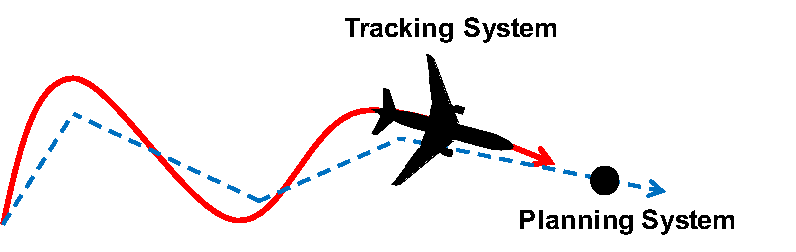
\includegraphics[width=0.35\textwidth]{fig/chasing}
	\caption{Left: A planning system (blue disk) using a fast but simple model, followed by a tracking system (green plane) using a more complex model, navigating through an environment with obstacles; the tracking system is guaranteed to stay within some TEB (blue circle). Right: Safety and goal-satisfaction can be guaranteed by planning with respect to augmented obstacles (large blue circles).}
	\label{fig:chasing}
\end{figure}
%

FaSTrack to be modular, and it can be used with any method for computing the TEB in conjunction with any existing fast path or trajectory planners, enabling motion planning that is real-time, guaranteed safe, and dynamically accurate. 
In this paper, we demonstrate this tool by computing the TEBs solving a Hamilton-Jacobi (HJ) partial differential equation (PDE), and using a different planning algorithm for each numerical example. 
In the three examples, we also consider different models for the tracking system and the planning system.
In the simulations, the system travels through a static environment with constraints defined, for example, by obstacles, while experiencing disturbances.
The constraints are only fully known through online sensing, for example, once obstacles are within the limited sensing region of the vehicle. 
Combining this TEB with real-time planners the system is able to safely plan and track a trajectory through the environment in real time. 
The planning algorithms used in our numerical examples are the fast sweeping method (FSM) \cite{Takei2013}, rapidly-exploring random trees (RRT) \cite{Kuffner2000,Kavraki1996}, and model-predictive control (MPC) \cite{Qin2003}.
% Introduction (.5-1p)
%%Tracking with quadrotors is a need
%%There exist methods that work in real time and methods that work for safety but not very many for both
%%Goal: combine both in a simple way

% !TEX root = tracking.tex
\section{Related Work \label{sec:relatedwork}}
Motion planning is a very active area of research in the controls and robotics communities \cite{Hoy2015}.  In this section we will discuss past work on path planning, kinematic planning, and dynamic planning.  A major current challenge is to find an intersection of robust, nonlinear, and real-time planning. 

There is a wealth of research in the area of sample-based path planning.  Planning methods like rapidly-exploring random trees (RRT) \cite{Kuffner2000}, probabilistic road maps (PRM) \cite{Kavraki1996}, and fast marching tree (FMT) \cite{Janson2015} can find collision-free paths through known or partially known environments.  These paths can then be smoothed with shortcut-based methods or turned into optimal motion plans \cite{Richter2016, Karaman2011, Kobilarov2012}.  These systems work well in many applications, but are not designed to be robust to model uncertainty or disturbances.

Motion planning for kinematic systems can also be accomplished through online trajectory optimization using methods such as TrajOpt \cite{Schulman2013} and CHOMP \cite{Ratliff2009}. These methods can work extremely well in many applications, but are generally challenging to implement for real-time nonlinear dynamic systems due to the computational load.

Model predictive control (MPC) has been a very successful method for dynamic trajectory optimization in both academia and industry \cite{Qin2003}.  However, combining speed, safety, and complex dynamics is a difficult balance to achieve. Using MPC for robotic and aircraft systems typically requires reducing the system complexity to take advantage of linear programming or mixed integer linear programming (MILP) \cite{Alexis2016, Bellingham2002, Vitus2008, Zeilinger2011, Richter2012}. Robustness in linear systems can be achieved using constraint tightening MPC to balance speed with safety \cite{Kuwata2007, Richards2006} or reference tracking \cite{DiCairano2016}. Nonlinear MPC is most often used on systems that evolve more slowly over time \cite{Diehl2002, Schildbach2016}, but there is active work to speed computation using Newton type methods and structure exploitation \cite{Diehl2009, Quirynen2015, Grune2011, Neunert2016}. Adding robustness to nonlinear MPC is being explored through algorithms based on minimax formulation and tube MPCs that bound output trajectories of a system with a tube around a nominal path (see survey paper \cite{Hoy2015} for references).
%speed nonlinear: Findeisen2007,Gupta2015, Torrisi2016

%learning through neural networks \cite{Yan2014}, 
%minimax \cite{Lofberg2003, Kumar2014}
% tube \cite{Mayne2011, Cannon2011, Kumar2014, Gao2014}

There are other methods of dynamic trajectory planning that manage to cleverly skirt the issue of solving for optimal trajectories online.  One such method works by storing a fixed precomputed set of trajectories called motion primitives that are then selected and composed together online.  This has been remarkably useful in many practical applications \cite{Gillula2010, Dey2016, Barry2016}, and there is impressive work on making these systems robust using funnels \cite{Majumdar2016}.  Another tactic for online dynamic trajectory planning involves the generation of several random trajectories at each waypoint, and then picking the best of those computed \cite{Kalakrishnan2011, Schwesinger2013, Krusi2015}.  This method works well in many applications, but is risky in its reliance on finding randomly-generated collision-free trajectories. 

There are also motion planning methods that are designed to be robust. Control barrier functions \cite{Xu2015, Ames2014} place inequality constraints in the control input that allow for dynamic trajectory planning as a quadratic program. New work in planning using contraction theory works by forming safe tubes online around a nominal dynamic trajectory \cite{Singh2017}.

Offline planners like Hamilton-Jacobi reachability analysis can find control policies and guarantees for nonlinear systems that avoid obstacles and are robust to bounded disturbances \cite{Mitchell05}.  However, this method can only approach real-time speed for very low-dimensional (1D-2D) systems. Although there has been work to speed up analysis by decomposing high-dimensional systems into smaller subsystems \cite{Chen2016a, Chen2016b}, dimensionality is still a common hurdle.

The work presented in this paper differs from the robust planning methods above because it is designed to be modular and easy to use in conjunction with a number of path and trajectory planners. Additionally, FASTrack can handle bounded external disturbances (e.g. wind) and work with both known and unknown environments with static obstacles. 
% Related Work (1p)
%%work on fast planning
%%work on safe planning
%%work on both
%%how ours is different

% !TEX root = tracking.tex
\section{Problem Formulation \label{sec:formulation}}
We seek to simultaneously plan and track a trajectory (or path converted to a trajectory) online in real time. Planning is done using a kinematic or dynamic planning model. Tracking is done by a tracking model representing the autonomous system. The environment may contain static obstacles that are either known a priori or can be observed by the system within a limited sensing range (see Section \ref{sec:online}).

\subsection{Tracking Model}
The tracking model represents the autonomous system dynamics, and in general may be nonlinear and high-dimensional. Let $\tstate$ represent the state variables of the tracking model, which evolves according to
\begin{equation}
\begin{aligned}
\label{eq:tdyn}
\dot{\tstate} = \tdyn(\tstate, \tctrl, \dstb), \tvar \in [0, \thor], \tstate \in \tset, \tctrl \in \tcset, \dstb \in \dset.
\end{aligned}
\end{equation}
We assume that the system dynamics $\tdyn : \tset\ \times\ \tcset \times \dset \rightarrow \tset$ are uniformly continuous, bounded, and Lipschitz continuous in $\tstate$ for fixed control $\tctrl$. The control function $\tctrl(\cdot)$ and disturbance function $\dstb(\cdot)$ are drawn from the following sets:
\begin{equation}
\begin{aligned}
\tctrl(\cdot) \in \tcfset(t) = \{\phi: [0, \thor] \rightarrow \tcset: \phi(\cdot) \text{ is measurable}\},\\
\dstb(\cdot) \in \dfset(t) = \{\phi: [0, \thor] \rightarrow \dset: \phi(\cdot) \text{ is measurable}\},
\end{aligned}
\end{equation}
where $\tcset, \dset$ are compact and $t\in[0, \thor]$ for some $T>0$. Under these assumptions there exists a unique trajectory solving (\ref{eq:tdyn}) for a given $\tctrl(\cdot) \in \tcset$ \cite{Coddington84}. The trajectories of (\ref{eq:tdyn}) that solve this ODE will be denoted as $\ttraj(\tvar; \tstate, \tvar_0, \tctrl(\cdot))$, where $\tvar_0,\tvar \in [0, \thor]$ and $\tvar_0 \leq \tvar$. These trajectories satisfy
\begin{equation}
\label{eq:fdyn_traj}
\begin{aligned}
\dot\ttraj(\tvar; \tstate, \tvar_0, \tctrl(\cdot)) &= \tdyn(\ttraj(\tvar; \tstate, \tvar_0, \tctrl(\cdot)), \tctrl(\tvar)), \\
\ttraj(\tvar; \tstate, \tvar, \tctrl(\cdot)) &= \tstate.
\end{aligned}
\end{equation}

\subsection{Planning Model}
The planning model is used by the path or trajectory planner to determine a desired path online. Kinematics or low-dimensional dynamics are typically used depending on the requirements of the planner. Let $\pstate$ represent the state variables of the planning model, with control $\pctrl$. The planning states $\pstate \in \pset$ are a subset of the tracking states $\tstate \in \tset$. The dynamics similarly satisfy 
\begin{equation}
\begin{aligned}
\label{eq:pdyn}
\dot{\pstate} = \pdyn(\pstate, \pctrl), \tvar \in [0, \thor], \pstate \in \pset, \ \underline{\pctrl} \leq \pctrl \leq \overline{\pctrl}.
\end{aligned}
\end{equation}
Note that the planning model does not involve a disturbance input. This is a key feature of FaSTrack: the treatment of disturbances is only necessary in the tracking model, which is modular with respect to any planning method, including those that do not account for disturbances.

\subsection{Goals of This Paper}
The goals of the paper are threefold:
\begin{enumerate}
	\item To provide a tool for precomputing functions (or look-up tables) to determine a guaranteed tracking error bound between tracking and planning models, and optimal safety controller for robust motion planning with nonlinear dynamic systems
	\item To develop a framework for easily implementing this tool with fast real-time path and trajectory planners.
	\item To demonstrate the tool and framework in an example using a high dimensional system
\end{enumerate}


% !TEX root = tracking.tex
\section{Computing Tracking Safety Radius \label{sec:reachability}}
Goals overview: Compute invariant sets, given by the optimization solution

Properties of solution: 

\subsection{Tracking as a Pursuit-Evasion Game}

\subsection{Optimization Problem}

\subsection{Dynamics of a Geometric Path}

\subsection{Solving the Optimization}

HJ Reachability (~1p)

Relative dynamics, setup, etc. (~1p)

Capture basin computation (~0.5p)
% Computing capture basin (~2.5p)
%% HJ Reachability (~1p)
%% Relative dynamics, setup, etc. (~1p)
%% Capture basin computation (~0.5p)

% !TEX root = tracking.tex
\section{Fast Path Planning using Rapidly-Exploring Random Tree \label{sec:rrt}}
Potential methods to use (~.5p)

Dealing with obstacles (~.5p)

% !TEX root = tracking.tex
\section{Fast Path Planning using Rapidly-Exploring Random Tree \label{sec:rrt}}
Potential methods to use (~.5p)

Dealing with obstacles (~.5p)
% Fast Path Planning using MPC (~1p)
%% Potential methods to use (~.5p)
%% Dealing with obstacles (~.5p)

% !TEX root = tracking.tex
\section{10D Quadrotor RRT Example \label{sec:results}}
\begin{figure*}
	\centering
	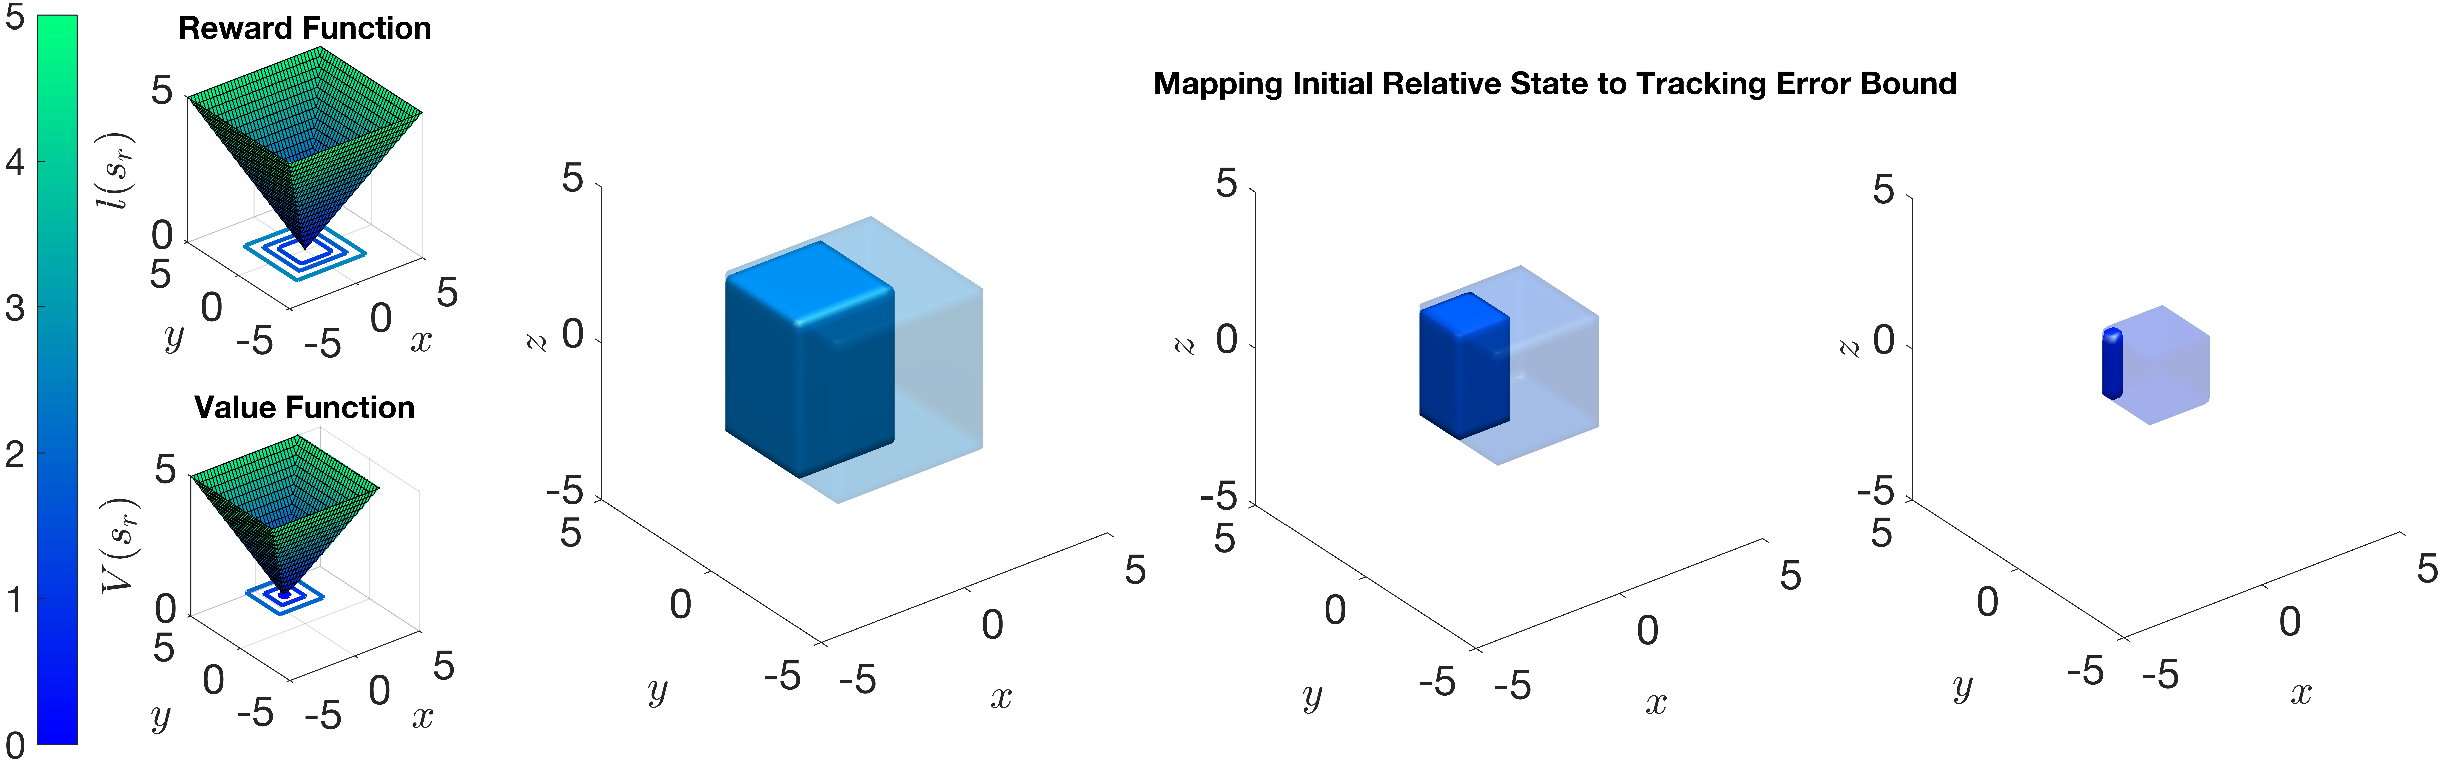
\includegraphics[width=0.9\textwidth]{fig/quad10D_example_cost}
	\caption{On the left are visualizations of the cost and value functions over a 2D slice of the 10D relative state space, with contour lines showing three level sets of these functions. The three images on the right show the 3D projections of these level sets at the same slice $(v_{xr},v_{yr},v_{zr})=[1, -1, 1]$ m/s, $(\theta_{xr},\omega_{xr},\theta_{yr},\omega_{yr})=[0,0,0,0]$. The solid boxes show the initial relative states, and the transparent boxes show the guaranteed tracking error bound around these relative states. In the online algorithm we will set the initial relative states to 0 to find the smallest invariant tracking error bound for the system.}
	\label{fig:quad10D_example}
	\end{figure*} 
\begin{figure}
	\centering
	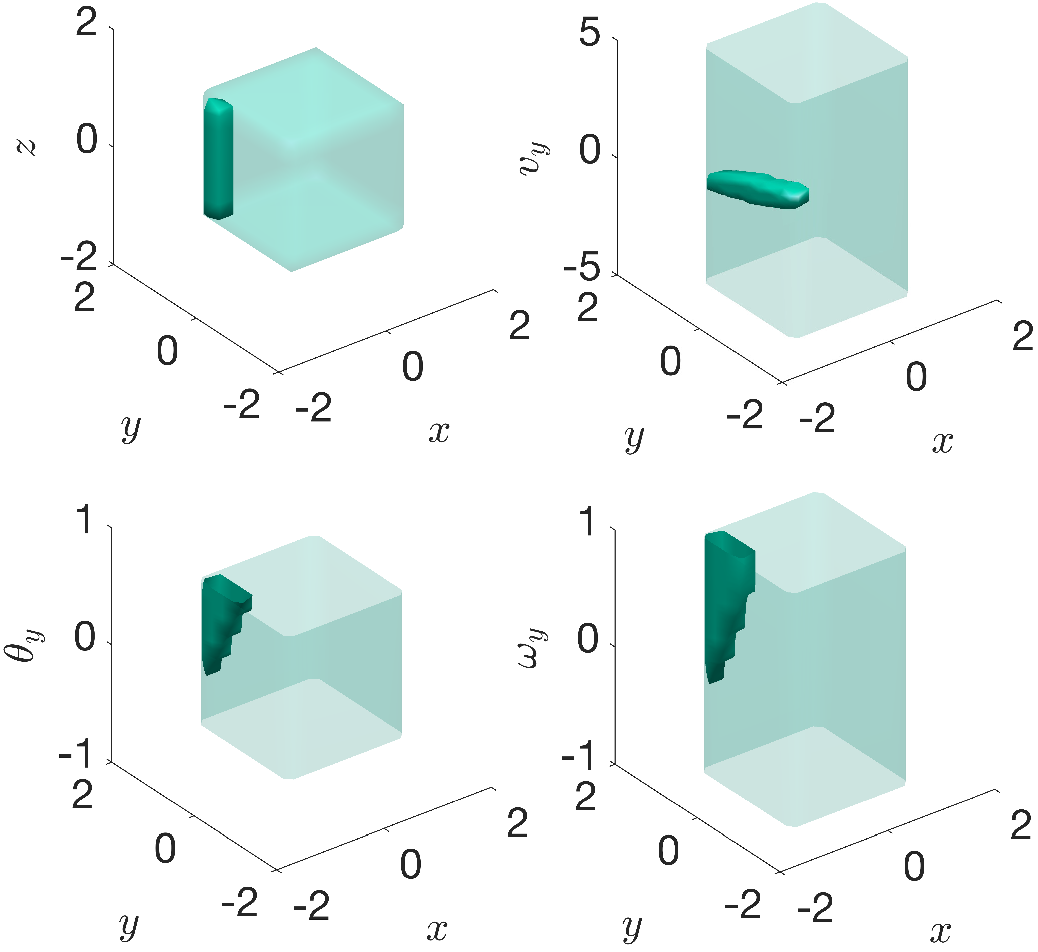
\includegraphics[width=0.3\textwidth]{fig/quad10D_slices}
	\caption{Various 3D slices along different dimensions of the 10D initial relative states (solid) and the corresponding tracking error bound (transparent)}
	\label{fig:quad10D_example_slices}
\end{figure} 
We demonstrate this framework with a 10D near-hover quadrotor developed in \cite{Bouffard12} tracking a 3D point source path generated by an RRT planner. First we perform the offline computations to acquire the tracking error bound and safety controller look-up tables. Next we set up the RRT to convert paths to simple 3D trajectories. Finally we implement the online framework to navigate the 10D system through a 3D environment with static obstacles.

\subsection{Precomputation of 10D-3D system}
First we define the 10D dynamics of the tracking quadrotor and the 3D dynamics of a holonomic vehicle:
\begin{equation}
\label{eq:Quad10D_dyn}
\begin{aligned}
\begin{array}{c}
\left[
\begin{array}{c}
\dot{x}\\
\dot{v_x}\\
\dot{\theta_x}\\
\dot\omega_x\\
\dot{y}\\
\dot{v_y}\\
\dot{\theta_y}\\
\dot\omega_y\\
\dot{z}\\
\dot{v_z}
\end{array}
\right]
=
\left[
\begin{array}{c}
v_x + d_x\\
g \tan \theta_x\\
-d_1 \theta_x + \omega_x\\
-d_0 \theta_x + n_0 a_x\\
v_y + d_y\\
g \tan \theta_y\\
-d_1 \theta_y + \omega_y\\
-d_0 \theta_y + n_0 a_y\\
v_z + d_z\\
k_T a_z - g
\end{array}
\right]
\left[
\begin{array}{c}
\dot{x}\\
\dot{y}\\
\dot{z}\\
\end{array}
\right], \quad
=
\left[
\begin{array}{c}
b_x\\
b_y\\
b_z \\
\end{array}
\right]
\end{array}\\
\end{aligned}
\end{equation}
where states $(x, y, z)$ denote the position, $(v_x, v_y, v_z)$ denote the velocity, $(\theta_x, \theta_y)$ denote the pitch and roll, and $(\omega_x, \omega_y)$ denote the pitch and roll rates. The controls of the 10D system are $(a_x, a_y, a_z)$, where $a_x$ and $a_y$ represent the desired pitch and roll angle, and $a_z$ represents the vertical thrust. The 3D system controls are $(b_x, b_y, b_z)$, and represent the velocity in each positional dimension. The disturbances in the 10D system $(d_x, d_y, d_z)$ are caused by wind, which acts on the velocity in each dimension. Next the relative dynamics between the two systems is defined using (\ref{eq:rdyn}):
\begin{equation}
\label{eq:Quad10DRel_dyn}
\begin{aligned}
\begin{array}{c}
\left[
\begin{array}{c}
\dot{x_r}\\
\dot{v_{xr}}\\
\dot{\theta_{xr}}\\
\dot\omega_{xr}\\
\dot{y_r}\\
\dot{v_{yr}}\\
\dot{\theta_{yr}}\\
\dot\omega_{yr}\\
\dot{z_r}\\
\dot{v_{zr}}
\end{array}
\right]
=
\left[
\begin{array}{c}
v_x - b_x + d_x\\
g \tan \theta_x\\
-d_1 \theta_x + \omega_x\\
-d_0 \theta_x + n_0 a_x\\
v_y - b_y + d_y\\
g \tan \theta_y\\
-d_1 \theta_y + \omega_y\\
-d_0 \theta_y + n_0 a_y\\
v_z - b_z + d_z\\
k_T a_z - g
\end{array}
\right]
\end{array}\\
\end{aligned}
\end{equation}
The values for parameters $d_0,d_1,n_0,k_T,g$ used were: $d_0=10,d_1=8,n_0=10,k_T=0.91,g=9.81$. The 10D control bounds were $|a_x|,|a_y|\leq10$ degrees, $0\leq a_z\leq 1.5g$ m/s$^{2}$. The 3D control bounds were $|b_x|,|b_y|,|b_z|\leq0.5$ m/s. The disturbance bounds were $|d_x|,|d_y|,|d_z|\leq0.1$ m/s.

Next we follow the setup described in section \ref{sec:precomp} to create a cost function, which we then evaluate using HJ reachability until convergence to produce the invariant value function as in (\ref{eq:valfunc}). Historically this 10D nonlinear relative system would be intractable for HJ reachability analysis, but using new methods in \cite{Chen2016b} we can decompose this system into 3 subsystems (one for each positional dimension). To do this we must also decompose the cost function, resulting in a one-norm instead of a two-norm. This cost function as well as the resulting value function can be seen projected onto the $x,y$ dimensions in Figure \ref{fig:quad10D_example}.

Figure \ref{fig:quad10D_example} also shows 3D positional projections of the mapping between initial relative state to maximum potential relative distance over all time (i.e. tracking error bound). If the real system starts exactly at the origin in relative coordinates, its tracking error bound will be a box of 0.81 meters in each direction. Slices of the 3D set and corresponding tracking error bounds are also shown in \ref{fig:quad10D_example_slices}. We save the look-up tables of the value function (i.e. the tracking error function) and its spatial gradients (i.e. the safety controller function).

\subsection{Online Planning with RRT and Sensing}
To demonstrate the combination of fast planning and provably robust tracking, we used a simple multi-tree RRT planner implemented in Matlab modified from \cite{Gavin2013}. We assigned a speed of $0.5$ m/s to the piecewise linear paths obtained from the RRT planner, so that the planning model is given in \eqref{eq:Quad10D_dyn}. Besides planning a path to the goal, the quadrotor must also sense obstacles in the vicinity. For illustration, we chose a simple virtual sensor that reveals obstacles within a range of 2 m in either the $x$, $y$, or $z$ direction.

Once an obstacle is sensed, the RRT planner replans while taking into account all obstacles that have been sensed so far. To ensure that the quadrotor does not collide with the obstacles despite error in tracking, planning is done with respect to augmented obstacles that are ``expanded'' from the sensed obstacles by $0.81$ m in the $x$, $y$, and $z$ directions.

On an unoptimized Matlab implementation on a desktop computer with a Core i7-2600K CPU, each iteration took a total of approximately $25$ ms on average. Most of this time is spent on planning: obtaining the tracking controller took approximately $5$ ms per iteration on average. The frequency of control was once every $100$ ms, so that path planning, obstacle sensing, and tracking are done in real-time.

Fig. \ref{fig:sim} shows the simulation results. Four time snapshots are shown. The starting point is $(-12, 0, 0)$, and the goal is marked by a circle. The gray planes are obstacles in the environment that have not yet been seen. The red color indicates the parts of the obstacles that have been seen. In all plots, a magenta star represents the position of the planning model; its movement is based on the paths planned by RRT, and is modeled by a 3D holonomic vehicle with a maximum speed. The blue box around the magenta star represents the tracking error bound.

The position of the tracking model is shown in blue. Throughout the simulation, the tracking model's position is always inside the tracking error, in agreement with Proposition \ref{prop:main}. In addition, the tracking error bound never intersects with the obstacles, a consequence of the RRT planner planning with respect to a set of augmented obstacles (not shown). In the latter two subplots, one can see that the quadrotor appears to be exploring the environment briefly before reaching the goal. In this paper, we did not employ any exploration algorithm; this exploration behavior is simply emerging from replanning using RRT whenever a new part (a $3$ m$^2$ portion) of an obstacle is sensed.

\begin{figure*}
  \centering
  \begin{subfigure}[t]{0.45\textwidth} \label{subfig:sim_1}
    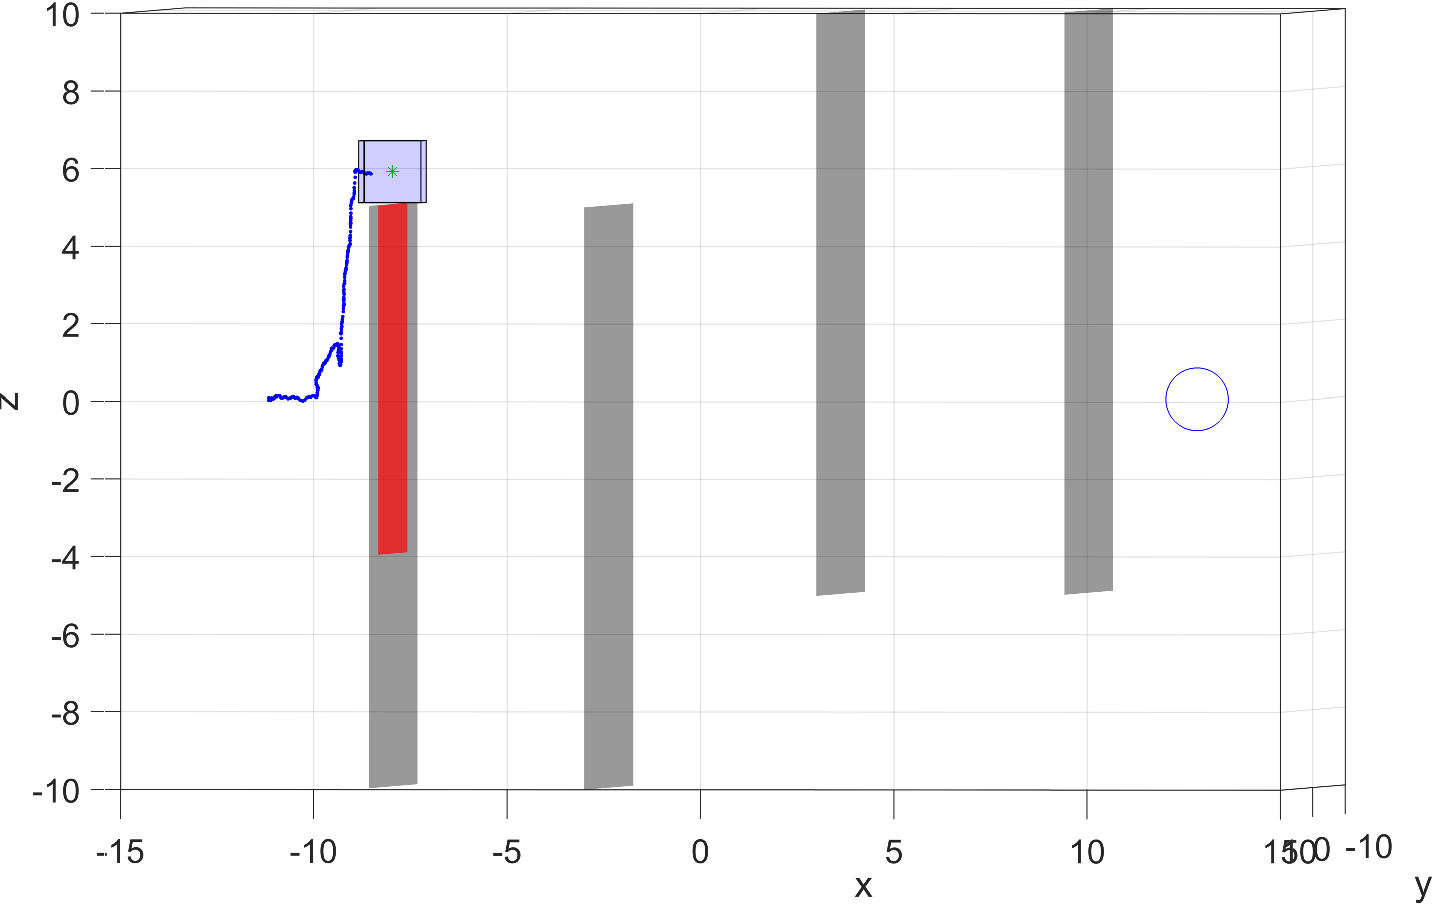
\includegraphics[width=\columnwidth]{fig/224}
    \caption{}
  \end{subfigure}
  \begin{subfigure}[t]{0.35\textwidth} \label{subfig:sim_2}
    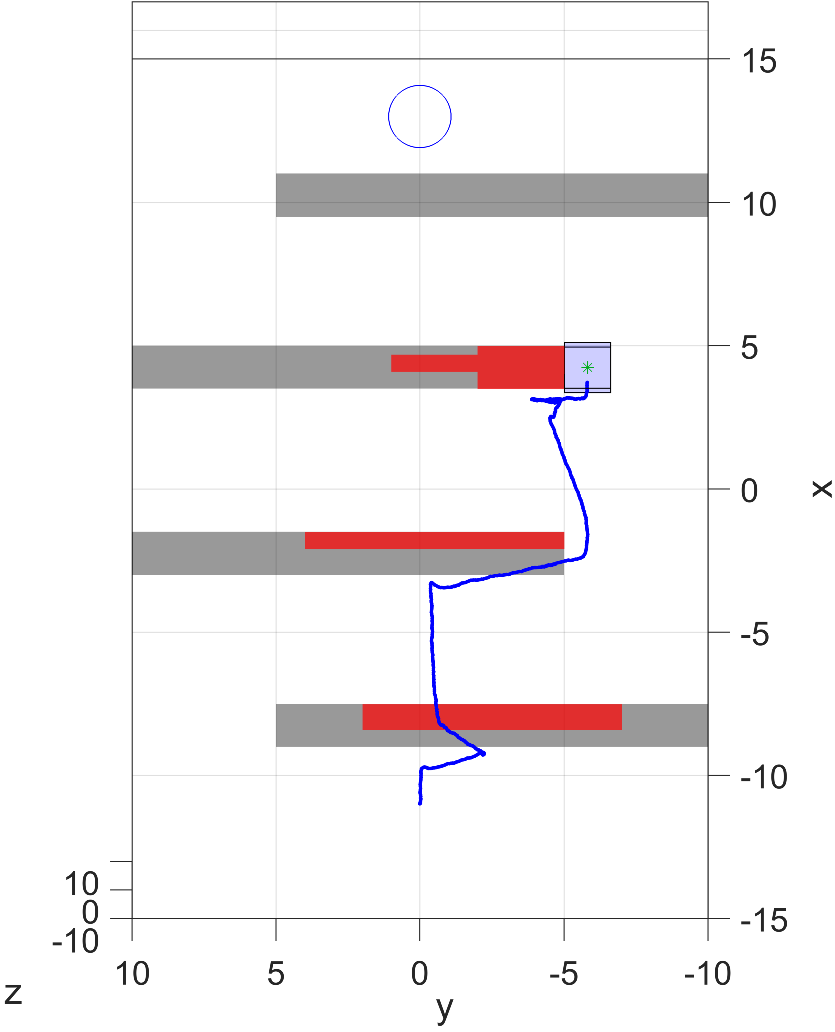
\includegraphics[width=\columnwidth]{fig/763}
    \caption{}
  \end{subfigure}
  
  \begin{subfigure}[t]{0.4\textwidth} \label{subfig:sim_3}
    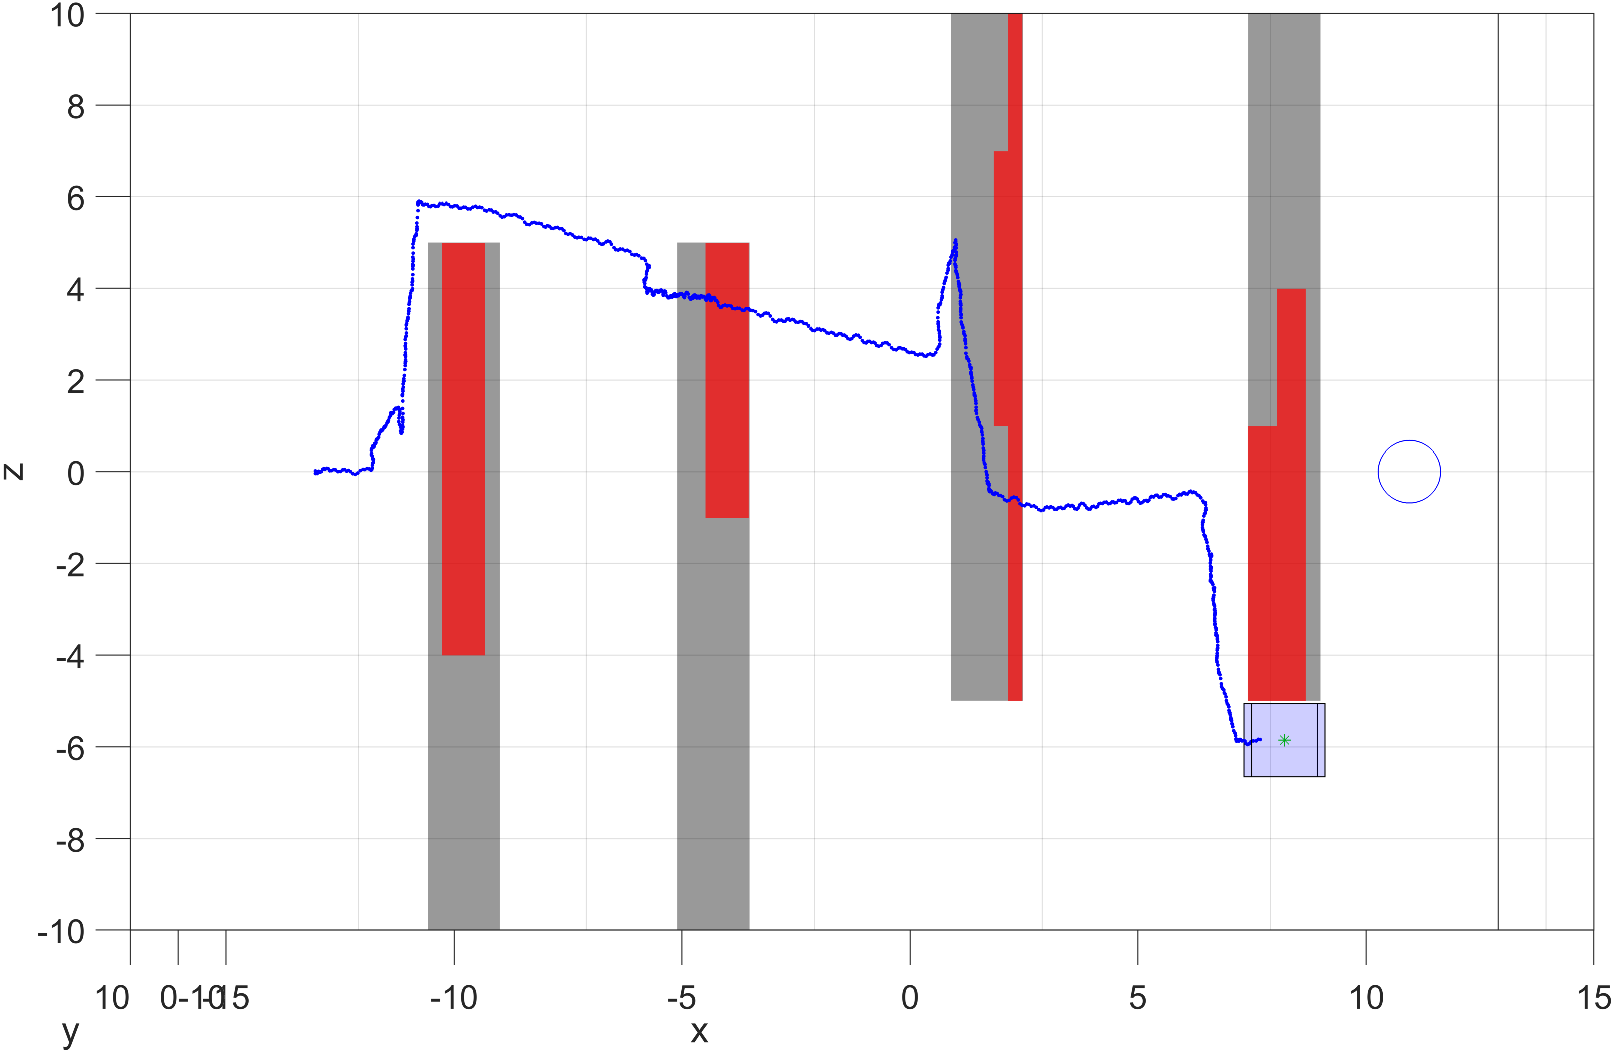
\includegraphics[width=\columnwidth]{fig/1042}
    \caption{}
  \end{subfigure}
  \begin{subfigure}[t]{0.4\textwidth} \label{subfig:sim_4}
    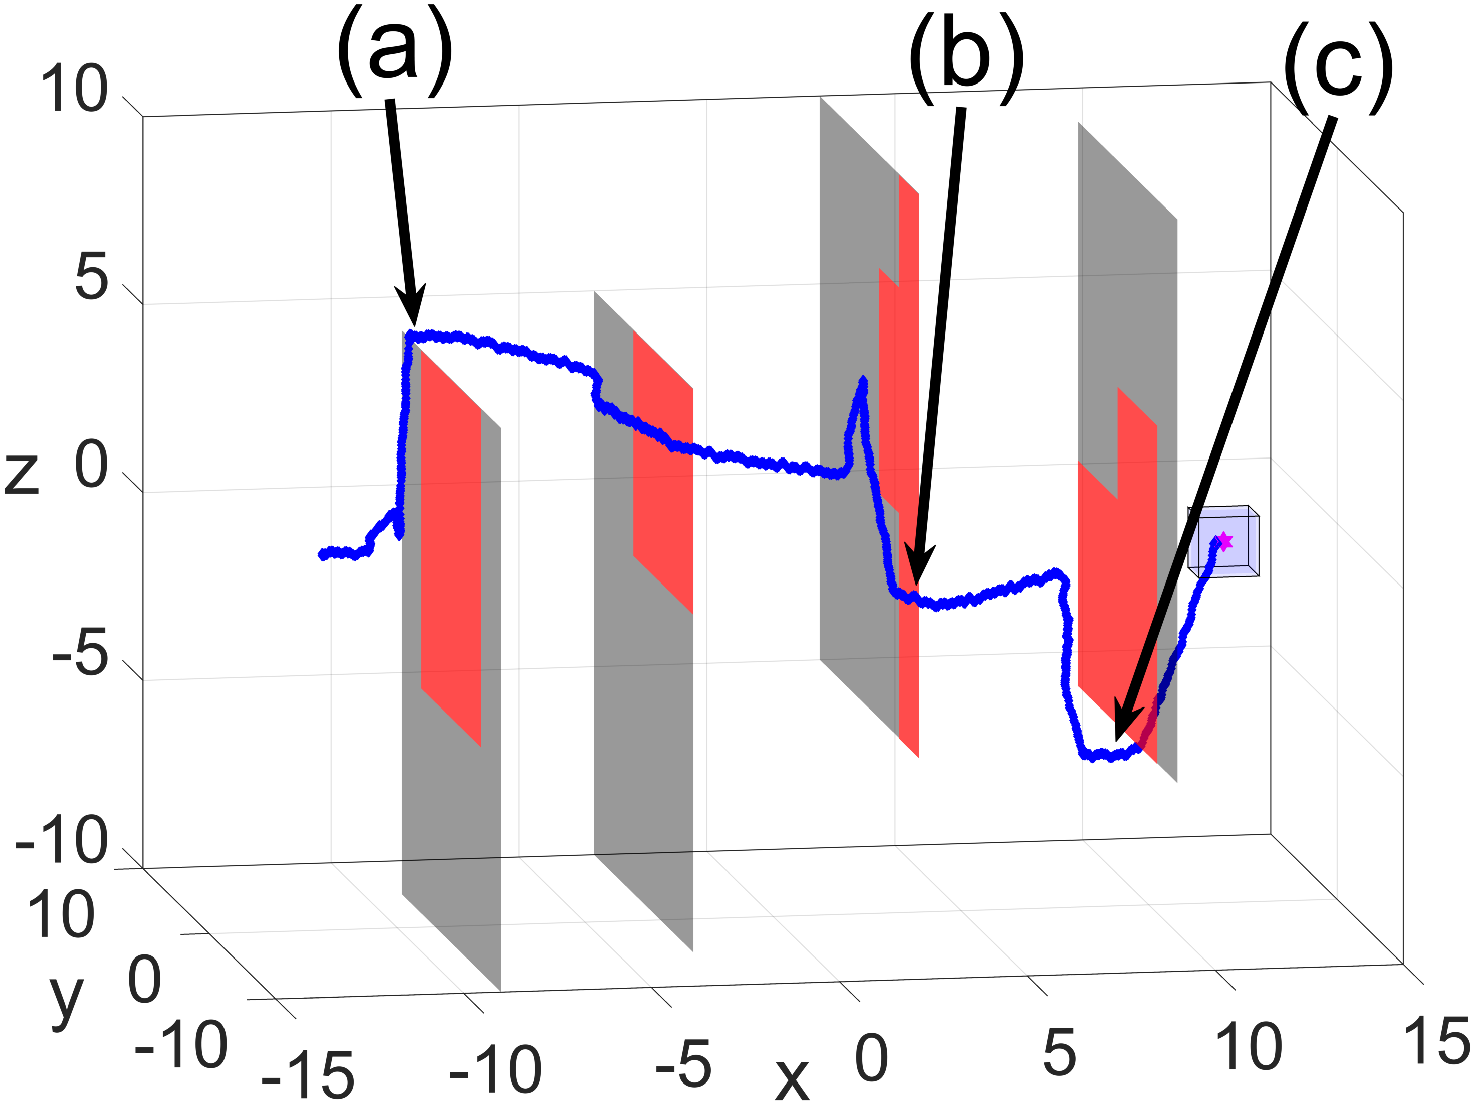
\includegraphics[width=\columnwidth]{fig/1173}
    \caption{}
  \end{subfigure}   
  \caption{A simulation showing how five vehicles initially in the Free mode can form a platoon. \label{fig:sim}}
\end{figure*}
% Numerical Simulations (1-2p)
%% demonstrate feasibility (~.5)
%% real-time computation load (~.5)
%% comparison to other methods (~.5)

% !TEX root = tracking.tex
\section{Conclusions and Future work}
In this paper we introduced our new tool FaSTrackHD: Fast and Safe Tracking for High Dimensional systems. This tool can be used to add robustness to various path and trajectory planners without sacrificing fast online computation. So far this tool can be applied to unknown environments with a limited sensing range and static obstacles. We are excited to explore several future directions for FaSTrackHD in the near future, including exploring robustness for moving obstacles, adaptable error bounds based on external disturbances, and demonstration on a variety of planners.
% Conclusion (0.5p)

%%%%%%%%%%%%%%%%%%%%%%%%%%%%%%%%%%%%%%%%%%%%%%%%%%%%%%%%%%%%%%%%%%%%%%%%%%%%%%%%
%\addtolength{\textheight}{1cm}   % This command serves to balance the column lengths
                                  % on the last page of the document manually. It shortens
                                  % the textheight of the last page by a suitable amount.
                                  % This command does not take effect until the next page
                                  % so it should come on the page before the last. Make
                                  % sure that you do not shorten the textheight too much.

\bibliographystyle{IEEEtran}
\bibliography{references}
\end{document}
